% Templ-MR architecture. Layers bottom to top: device, SDKs, app modules, network wrappers.
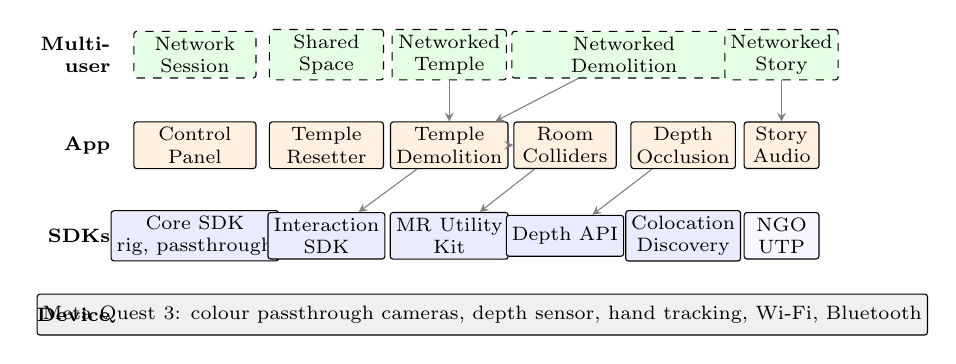
\begin{tikzpicture}[
  font=\scriptsize,
  layer/.style={draw, rounded corners=1pt, minimum height=5.2mm, inner sep=2pt, align=center},
  dev/.style={layer, fill=gray!12},
  sdk/.style={layer, fill=blue!8},
  app/.style={layer, fill=orange!12},
  net/.style={layer, fill=green!10, dashed},
  lbl/.style={font=\scriptsize\bfseries, anchor=east, align=right},
  >=stealth
]
% Device layer
\node[dev, minimum width=8.6cm] (dev) at (0.3,0)
  {Meta Quest 3: colour passthrough cameras, depth sensor, hand tracking, Wi-Fi, Bluetooth};
% SDK layer
\node[sdk, minimum width=1.55cm] (core) at (-3.35,1.0) {Core SDK\\rig, passthrough};
\node[sdk, minimum width=1.45cm] (isdk) at (-1.68,1.0) {Interaction\\SDK};
\node[sdk, minimum width=1.45cm] (mruk) at (-0.12,1.0) {MR Utility\\Kit};
\node[sdk, minimum width=1.30cm] (depth) at (1.35,1.0) {Depth API};
\node[sdk, minimum width=1.30cm] (coloc) at (2.85,1.0) {Colocation\\Discovery};
\node[sdk, minimum width=0.95cm, fill=blue!3] (ngo) at (4.1,1.0) {NGO\\UTP};
% App layer
\node[app, minimum width=1.55cm] (panel) at (-3.35,2.15) {Control\\Panel};
\node[app, minimum width=1.45cm] (reset) at (-1.68,2.15) {Temple\\Resetter};
\node[app, minimum width=1.45cm] (demo) at (-0.12,2.15) {Temple\\Demolition};
\node[app, minimum width=1.30cm] (room) at (1.35,2.15) {Room\\Colliders};
\node[app, minimum width=1.30cm] (occ) at (2.85,2.15) {Depth\\Occlusion};
\node[app, minimum width=0.95cm] (story) at (4.1,2.15) {Story\\Audio};
% Network layer
\node[net, minimum width=1.55cm] (sess) at (-3.35,3.3) {Network\\Session};
\node[net, minimum width=1.45cm] (space) at (-1.68,3.3) {Shared\\Space};
\node[net, minimum width=1.45cm] (ntemple) at (-0.12,3.3) {Networked\\Temple};
\node[net, minimum width=2.85cm] (ndemo) at (2.1,3.3) {Networked\\Demolition};
\node[net, minimum width=0.95cm] (nstory) at (4.1,3.3) {Networked\\Story};
% Layer labels
\node[lbl] at (-4.3,0) {Device};
\node[lbl] at (-4.3,1.0) {SDKs};
\node[lbl] at (-4.3,2.15) {App};
\node[lbl] at (-4.3,3.3) {Multi-\\user};
% Key dependencies between adjacent layers only, so no arrow crosses a box.
% Not drawn: NetworkSession uses Colocation Discovery and NGO; SharedSpace uses MRUK.
\draw[->, gray] (demo) -- (isdk);
\draw[->, gray] (room) -- (mruk);
\draw[->, gray] (occ) -- (depth);
\draw[->, gray] (ndemo) -- (demo);
\draw[->, gray] (ntemple) -- (demo);
\draw[->, gray] (nstory) -- (story);
\draw[->, gray] (demo) -- (room);
\end{tikzpicture}
